\chapter{General problem description}
Indoor tracking is a very complex matter because the common GPS system is unvailable due to the fact that satellite signals are often absent or very imprecise inside buildings.
From that very fact came the need to research other resources that coud provide location.
In fact many research labs and companies are developing solutions based on Wi-Fi signals triangulation although this kind of systems are too imprecise for our purpose due too many facts, such as: signal loss,latency, continuos connect and disconnect from a range of Wi-fi hotspots in order to measure the singal intesity.
In addition, a wireless solution will impact the autonomy of the device and the installation of Wi-Fi repetitors might be a burden for the final user.
\newline
A marker, which is basically a symbol, avoids all those problems although it brings another level of complexity by introducing other matters, such as: recognize of the symbol, how to read the data, quantity of information, where it should stand.
All this problems plus some other will be analized in the folowing sections.

\subsection{QR Code quick generalities}
A QRCode is foundamentally an image containing an encoded binary matrix of data which displays like:
\begin{figure}[hbt]
    \centering
    \caption{A generic QrCode}
    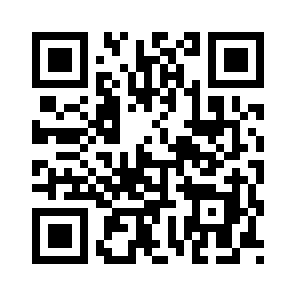
\includegraphics[scale=0.5]{img/qr.png}
\end{figure}

There are 41 versions of it and they differ from each other by their matrix 
module size which is fixed for each version and ranges from a minimum of 21x21 
to a maximum of 177x177. This allows to save up to 23648 bits.\footnote{with an L level or error correction} 
\newline 
In addition, the encoding algorithm\footnote{ according to: \url{http://raidenii.net/files/datasheets/misc/qr_code.pdf}} offers the opportunity of error correction through the usage of Reed-Solomon codes.
These codes are also stored inside the QR Code and the there are four levels of error recovering which can be choosen by the user according to the operating environment.
In fact, each level increases its capability of restoring data but also require more space on the QR Code's matrix in order to work. 
\newpage
To simplify the above description here's a summarying table:
\begin{figure}[hbt]
    \centering
    \caption{Versions of QRCode \protect \footnote{complete table at: \protect \url{http://www.qrcode.com/en/about/version.html}}}
    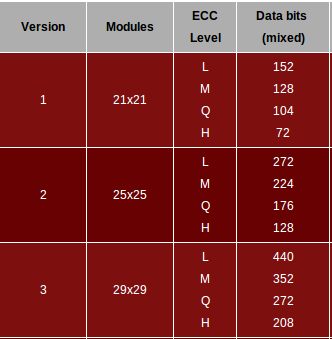
\includegraphics[scale=0.9]{img/qrversion.png}
\end{figure}


   













  
